\chapter{Results}\label{ch:results}

All numbers in this chapter are the highest ambiguity of \cref{sec:metric}, in dB relative to the peak of the reference.
Every method receives only the system parameters and the DEM. The scenes cover along-track ramps (\SIrange{3}{20}{\degree}),
sines and cosines of several periods, and realistic terrains (hills, mountains, escarpments, plateaus, fractal alpine relief,
glacial valleys, ridges, canyons, volcanoes), each with one, a few and many point targets (up to 49). The baselines are
$\Nrx=2,3,4,6,8$ with $\bxt^{\max}=\SIlist{100;300;500}{m}$ (random, the largest exactly $\bxt^{\max}$), plus five fixed
four-channel sets: two random ones (up to \SI{100}{m} and up to \SI{500}{m}), two equally spaced ones ($[0,10,20,30]$ and
$[0,50,100,150]$\,\si{m}) and one with baselines on both sides of the transmitter ($[0,-50,50,100]$\,\si{m}). Channel~0 is always the transmitter.

\section{All methods with a DEM only}\label{sec:audit}

\Cref{tab:audit,fig:audit} compare the methods on \AuditRuns{} runs (\AuditScenes{} scenes $\times$ 20 baseline sets;
median reference \SI{\AuditMedRef}{dB}).

\begin{table}[htbp]
\centering
\caption[Comparison of all methods]{All methods with the DEM only (\AuditRuns{} runs).}
\label{tab:audit}
\begin{tabular}{@{}l >{\centering\arraybackslash}p{3.0cm} >{\centering\arraybackslash}p{3.2cm}@{}}
\toprule
Method & Median highest ambiguity [dB] & Runs within \SI{10}{dB} of the reference [\%] \\
\midrule
No correction (standard reconstruction) & $-8.7$ & 3.5 \\
SATA whole band, then reconstruction & $-15.4$ & 2.5 \\
SATA per sub-band & $-10.8$ & 1.2 \\
Joint reconstruction in the sub-apertures & $-30.9$ & 36.3 \\
\textbf{Joint reconstruction over the whole line} & $\mathbf{-41.4}$ & \textbf{81.9} \\
\bottomrule
\end{tabular}
\end{table}

\begin{figure}[htbp]
\centering
\begin{tikzpicture}
\begin{axis}[
  width=0.75\linewidth, height=6cm, ybar, bar width=16pt,
  ymin=-50, ymax=0, ylabel={median highest ambiguity [dB]},
  xtick={0,1,2,3,4},
  xticklabels={{no\\correction},{SATA\\whole band},{SATA per\\sub-band},{joint\\sub-apertures},{joint\\whole line}},
  xticklabel style={align=center,font=\small},
  nodes near coords, nodes near coords style={font=\scriptsize,anchor=north,yshift=-2pt,/pgf/number format/fixed,/pgf/number format/precision=1},
  ymajorgrids, grid style={gray!25}, enlarge x limits=0.15]
  \addplot[fill=cjoint!60,draw=cjoint] table[x=idx,y=median] {data/audit_methods.dat};
  \draw[cref,thick,dashed] (axis cs:-0.5,\AuditMedRef) -- (axis cs:4.5,\AuditMedRef) node[pos=0.02,above,anchor=south west,font=\scriptsize]{reference (median)};
\end{axis}
\end{tikzpicture}
\caption[Median highest ambiguity of every method]{Median highest ambiguity of every method over the \AuditRuns{} runs of
the audit. SATA per channel stays close to the uncorrected reconstruction; the joint reconstruction over the whole line
gets within a few dB of the reference.}
\label{fig:audit}
\end{figure}

Head to head, the joint reconstruction over the whole line is better than SATA whole band in all \AuditRuns{} runs
(median improvement \SI{\AuditLineBetterWhole}{dB}) and better than SATA per sub-band in all of them (median
\SI{\AuditLineBetterSub}{dB}). SATA per channel improves on the uncorrected reconstruction by a median of only \SI{5.5}{dB}
(whole band) and \SI{0.2}{dB} (per sub-band), consistently with \cref{sec:sata-limit}.

A distributed scene (about \num{11900} scatterers, oracle \SI{-34.2}{dB}, measured as error-to-signal ratio) confirms the
ranking: with $\bxt\sim U(0,100)$\,\si{m} SATA per channel gives \SIrange{-22.5}{-8.7}{dB} and the whole-line joint
\SIrange{-34.1}{-33.2}{dB}; with $U(0,500)$\,\si{m}, \SIrange{-13}{-6}{dB} and \SIrange{-33.6}{-31.4}{dB}.

\section{Why the joint reconstruction is the final method}\label{sec:whyjoint}

\Cref{fig:satavsjoint} compares all the methods on one realistic scene: five targets on random mountains (relief \SI{1000}{m}),
four channels with $\bxt^{\max}=\SI{300}{m}$. No SATA leaves \SI{-4.6}{dB}; SATA whole band \SI{-14.6}{dB}; SATA per sub-band
\SI{-8.6}{dB}; the joint reconstruction over the whole line \SI{-43.6}{dB}, \SI{5}{dB} from the reference (\SI{-48.7}{dB}).
\Cref{fig:auditscatter} shows that this is not a particular case: over the \AuditRuns{} runs of the audit the joint reconstruction
is better than SATA in every run, by a median of \SI{\AuditLineBetterWhole}{dB} (whole band) and \SI{\AuditLineBetterSub}{dB} (per
sub-band).

\begin{figure}[htbp]
\centering
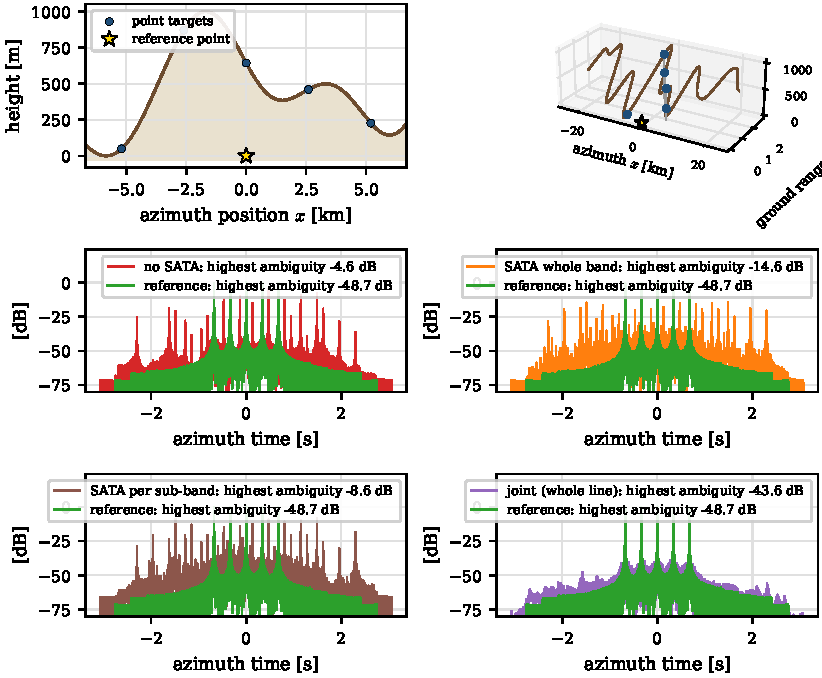
\includegraphics[width=\linewidth]{figures/sata_vs_joint_mountains.pdf}
\caption[All the methods on a realistic scene]{Five targets \SI{2.6}{km} apart on random mountains (relief \SI{1000}{m},
correlation length \SI{3}{km}), four channels, $\bxt=[0,300,119.8,100.5]$\,\si{m}. Top: the targets and the terrain near them
(left) and along the whole azimuth line (right). Below: impulse responses of the reference and of no SATA, SATA whole band, SATA
per sub-band and the joint reconstruction over the whole line. Every method reads only the DEM.}
\label{fig:satavsjoint}
\end{figure}

\begin{figure}[htbp]
\centering
\begin{tikzpicture}
\begin{groupplot}[group style={group size=2 by 1, horizontal sep=1.5cm},
  width=0.46\linewidth, height=0.46\linewidth, xmin=-75, xmax=15, ymin=-75, ymax=15,
  ylabel={joint (whole line) [dB]}, grid=major, grid style={gray!20},
  scatter/classes={2={mark=*,cnone,mark size=0.8pt}, 3={mark=*,cwhole,mark size=0.8pt}, 4={mark=*,cjoint,mark size=0.8pt},
                   6={mark=*,cocc,mark size=0.8pt}, 8={mark=*,cref,mark size=0.8pt}},
  legend style={font=\scriptsize,draw=none,fill=white,fill opacity=0.85,text opacity=1}, legend pos=north west]
\nextgroupplot[xlabel={SATA whole band [dB]}]
  \addplot[scatter,only marks,scatter src=explicit symbolic,opacity=0.6] table[x=whole,y=line,meta=nrx] {data/audit_scatter.dat};
  \addplot[gray,dashed,domain=-75:15] {x};
  \legend{$\Nrx=2$,3,4,6,8}
\nextgroupplot[xlabel={SATA per sub-band [dB]}, ylabel={}]
  \addplot[scatter,only marks,scatter src=explicit symbolic,opacity=0.6] table[x=sub,y=line,meta=nrx] {data/audit_scatter.dat};
  \addplot[gray,dashed,domain=-75:15] {x};
\end{groupplot}
\end{tikzpicture}
\caption[SATA against the joint reconstruction, every run]{Highest ambiguity of the joint reconstruction over the whole line
against SATA whole band (left) and SATA per sub-band (right), for the \AuditRuns{} runs of the audit (every method with the DEM
only), coloured by the number of channels. Every point is below the diagonal.}
\label{fig:auditscatter}
\end{figure}

The reasons, collected from the previous chapters:
\begin{enumerate}
  \item \textbf{SATA has the right phase in the wrong place.} SATA reads the correct correction, the $\Delta C_0$ of the DEM. But
        on an aliased channel each bin is the sum of parcels from positions $X\approx\SI{6.2}{km}$ apart, and a per-channel
        correction can give that sum only one phase (\cref{fig:binconflict}). The standard reconstruction that follows assumes that
        every channel is now exact, so the error of the other parcels becomes leakage between the parcels. SATA is exact only when the
        terrain has the same height at all the folded positions (\cref{fig:satacontrols}), it can damage a target that needed no
        correction (\cref{fig:satarefpoint}), and the level it leaves is predicted by the geometry (\cref{fig:sataprediction}): it is a
        property of the order of the operations, not of the implementation. Applying SATA after the reconstruction does not help
        either, since one phase cannot undo a sum that has already been formed.
  \item \textbf{The joint reconstruction solves both problems together.} Separating the parcels needs the phases corrected, and
        correcting each parcel needs the parcels separated. The joint reconstruction writes the phase of every ground position
        \emph{inside} the model of the channels (\cref{fig:pipelines}) and inverts model and topography together. With a flat DEM it is
        the standard reconstruction; on the periodic terrains where SATA is exact it gives the same result as SATA; everywhere else it
        keeps working.
  \item \textbf{The whole-line version removes the last approximation.} The joint reconstruction in the sub-apertures still reads
        the DEM once per bin of a \SI{40}{ms} block, i.e.\ it takes the terrain phase as constant over about $\pm\SI{600}{m}$, and fails
        on steep terrain with long baselines (median \SI{-30.9}{dB} in the audit). Over the whole line the residual of every
        scatterer is a pointwise phase on the focused line, with no cell at all (median \SI{-41.4}{dB}).
  \item \textbf{It uses only what a real case has.} The method receives the channels, the system geometry and the DEM; the
        positions of the targets are never used, and the unexplained part of the channels gives a check of the DEM.
  \item \textbf{It degrades gracefully.} Where the baselines do not separate the parcels the regularisation leaves the ambiguity
        instead of amplifying noise, and the cost (a few seconds per line in the 1-D simulator) is that of a few tens of FFTs per
        channel and iteration.
\end{enumerate}

\section{Sweep of the final joint reconstruction in 1-D}\label{sec:sweep1d}

The complete 1-D sweep runs the reference, the uncorrected reconstruction and
the joint reconstruction over the whole line on \SweepOneScenes{} scenes $\times$ 20 baseline sets = \SweepOneRuns{} runs.
The medians are \SI{\SweepOneMedRef}{dB} (reference), \SI{\SweepOneMedNone}{dB} (no correction) and
\SI{\SweepOneMedJoint}{dB} (joint); \SweepOneWithinTen\,\% of the runs are within \SI{10}{dB} of the reference.
\Cref{fig:nrx1d} splits the result by the number of channels and \cref{fig:scatter} shows every run.

\begin{figure}[htbp]
\centering
\begin{tikzpicture}
\begin{groupplot}[group style={group size=2 by 1, horizontal sep=1.8cm},
  width=0.47\linewidth, height=5.6cm, xtick={2,3,4,6,8}, xlabel={$\Nrx$},
  ymajorgrids, grid style={gray!25}, legend style={font=\scriptsize,draw=none,fill=white,fill opacity=0.85,text opacity=1}]
\nextgroupplot[ylabel={median highest ambiguity [dB]}, ymin=-60, ymax=0, legend style={at={(0.97,0.62)},anchor=east}]
  \addplot[cref,thick,mark=*] table[x=nrx,y=medref] {data/sweepone_nrx.dat};
  \addplot[cnone,thick,mark=square*,dashed] table[x=nrx,y=mednone] {data/sweepone_nrx.dat};
  \addplot[cjoint,thick,mark=triangle*] table[x=nrx,y=medjoint] {data/sweepone_nrx.dat};
  \legend{reference, no correction, joint}
\nextgroupplot[ylabel={runs within the margin [\%]}, ymin=0, ymax=100, legend pos=south east]
  \addplot[cjoint,thick,mark=triangle*] table[x=nrx,y=within10] {data/sweepone_nrx.dat};
  \addplot[cjoint!50,thick,mark=o] table[x=nrx,y=within3] {data/sweepone_nrx.dat};
  \legend{within \SI{10}{dB}, within \SI{3}{dB}}
\end{groupplot}
\end{tikzpicture}
\caption[1-D sweep by number of channels]{1-D sweep by number of channels. Left: medians of the highest ambiguity. Right:
fraction of runs in which the joint reconstruction is within \SI{10}{dB} and \SI{3}{dB} of the reference. The reference
level rises with $\Nrx$ because $\PRFop$ falls and more ambiguity orders fall inside the band.}
\label{fig:nrx1d}
\end{figure}

\begin{figure}[htbp]
\centering
\begin{tikzpicture}
\begin{groupplot}[group style={group size=2 by 1, horizontal sep=1.6cm},
  width=0.48\linewidth, height=0.48\linewidth, xmin=-75, xmax=15, ymin=-75, ymax=15,
  xlabel={no correction [dB]}, grid=major, grid style={gray!20},
  scatter/classes={2={mark=*,cnone,mark size=0.9pt}, 3={mark=*,cwhole,mark size=0.9pt}, 4={mark=*,cjoint,mark size=0.9pt},
                   6={mark=*,cocc,mark size=0.9pt}, 8={mark=*,cref,mark size=0.9pt}},
  legend style={font=\scriptsize,draw=none,fill=white,fill opacity=0.85,text opacity=1}, legend pos=north west]
\nextgroupplot[ylabel={joint reconstruction [dB]}, title={\small 1-D (\SweepOneRuns{} runs)}]
  \addplot[scatter,only marks,scatter src=explicit symbolic,opacity=0.6] table[x=none,y=joint,meta=nrx] {data/sweepone_scatter.dat};
  \addplot[gray,dashed,domain=-75:15] {x};
  \legend{$\Nrx=2$,3,4,6,8}
\nextgroupplot[title={\small 2-D (\SweepTwoRuns{} runs)}]
  \addplot[scatter,only marks,scatter src=explicit symbolic,opacity=0.6] table[x=none,y=joint,meta=nrx] {data/sweeptwo_scatter.dat};
  \addplot[gray,dashed,domain=-75:15] {x};
\end{groupplot}
\end{tikzpicture}
\caption[Every run of the sweeps]{Every run of the 1-D and 2-D sweeps: highest ambiguity of the joint reconstruction
against the uncorrected reconstruction, coloured by the number of channels. Points below the diagonal are improvements.}
\label{fig:scatter}
\end{figure}

The \SweepOneUnresolved{} runs that are not resolved (above \SI{-30}{dB} and more than \SI{10}{dB} from the reference)
are almost all configurations whose baselines cannot separate the parcels: 53 have two channels and 25 the equally spaced baselines
$[0,50,100,150]$\,\si{m}; only 5 have four random baselines (3 with $\bxt^{\max}=\SI{300}{m}$, 2 with \SI{500}{m}). \Cref{fig:alpine} shows a
typical resolved case on a fractal alpine relief. \Cref{fig:jointnrx} shows the role of the number of channels on one scene with
49 targets on random mountains and $\bxt^{\max}=\SI{300}{m}$: with three or more channels the joint reconstruction is within
\SIrange{1}{4}{dB} of the reference; with two channels there is no redundancy and it stops at \SI{-22.3}{dB} (reference
\SI{-38.5}{dB}), still \SI{8}{dB} better than no SATA.

\begin{figure}[htbp]
\centering
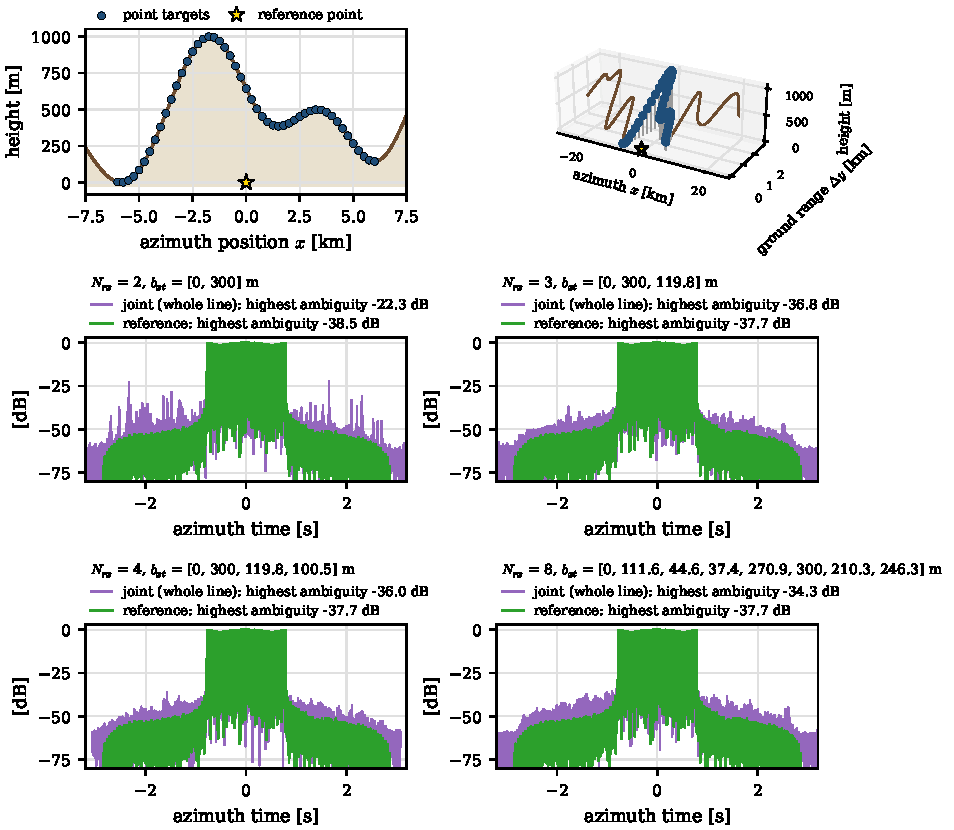
\includegraphics[width=\linewidth]{figures/joint_nrx_mountains49.pdf}
\caption[Joint reconstruction with 2, 3, 4 and 8 channels]{49 targets \SI{250}{m} apart on random mountains (relief
\SI{1000}{m}), largest cross-track baseline \SI{300}{m}, channel~0 on the transmitter. Top: the targets and the terrain near them
(left) and along the whole azimuth line (right). Below: impulse responses of the reference and of the joint reconstruction over the
whole line for $\Nrx=2$, 3, 4 and 8.}
\label{fig:jointnrx}
\end{figure}

\begin{figure}[p]
\centering
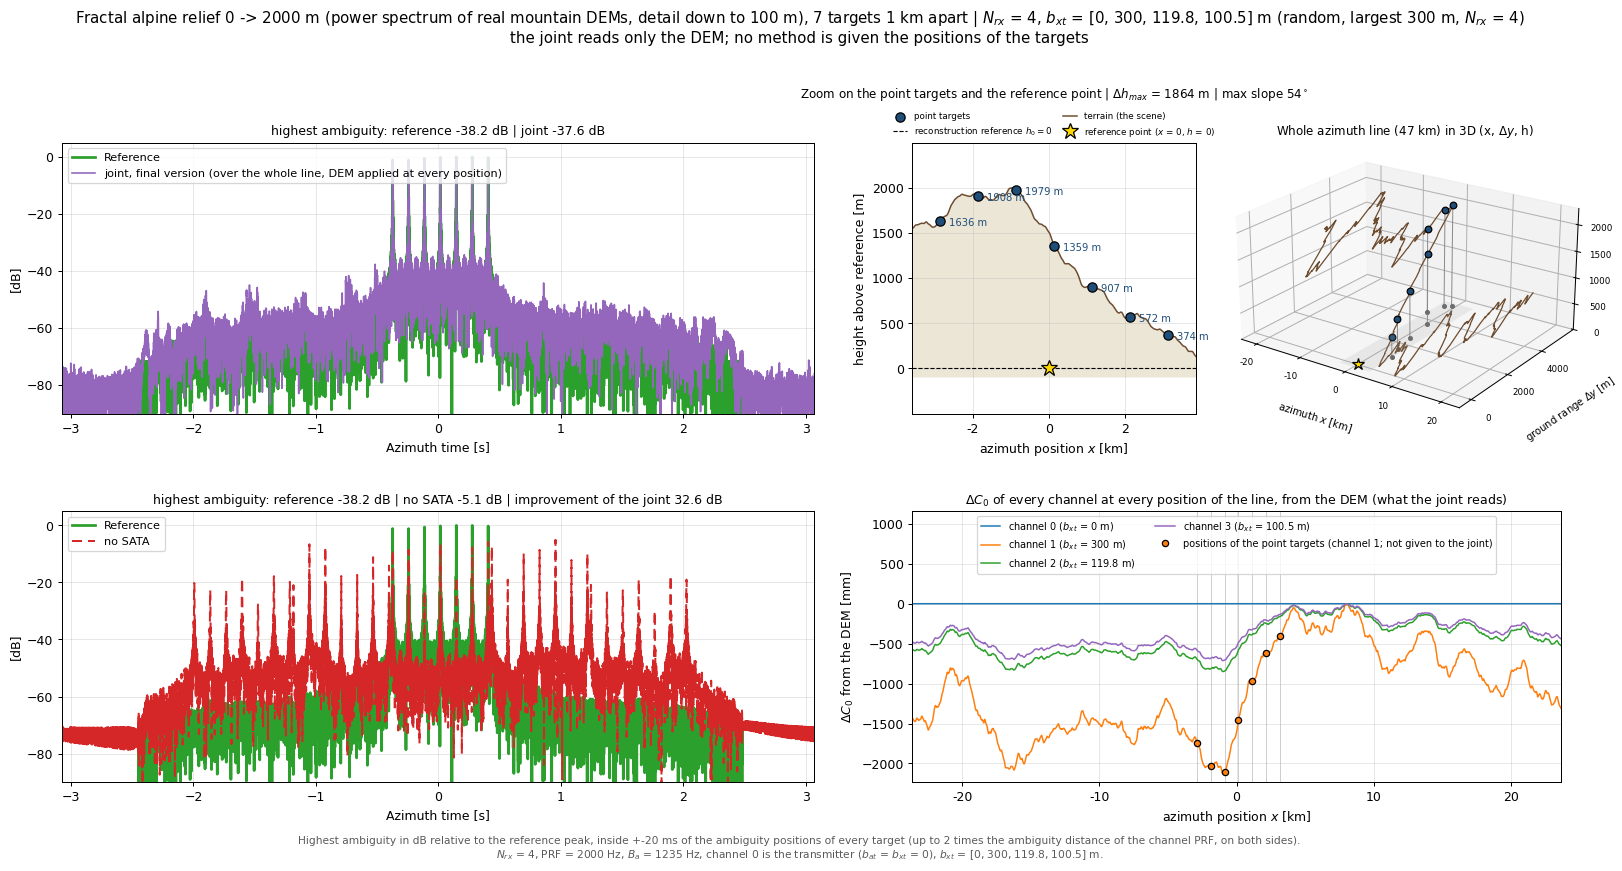
\includegraphics[width=\linewidth]{figures/sweep1d_alpine7_N4b300.png}
\caption[Example of the 1-D sweep]{A page of the 1-D sweep: seven targets on a fractal alpine relief (\SIrange{0}{2000}{m},
slopes up to \SI{54}{\degree}), $\Nrx=4$, $\bxt=[0,300,119.8,100.5]$\,\si{m}. The joint reconstruction (top left) reaches the
reference level (\SI{-37.6}{dB} against \SI{-38.2}{dB}); without correction the highest ambiguity is \SI{-5.1}{dB}. Bottom right:
the $\dC$ of every channel along the whole line, read from the DEM.}
\label{fig:alpine}
\end{figure}

\section{Sweep of the joint reconstruction in 2-D}\label{sec:sweep2d}

The 2-D sweep uses \SweepTwoScenes{} 3-D scenes (ramps along azimuth, range
and oblique; sines and cosines; realistic and fractal terrains without layover; one target on a flank, five on a diagonal or a
$7\times7$ grid) with the same 20 baseline sets, \SweepTwoRuns{} runs in total. The medians are \SI{\SweepTwoMedRef}{dB}
(reference), \SI{\SweepTwoMedNone}{dB} (no correction) and \SI{\SweepTwoMedJoint}{dB} (joint), all in the common range band.
The joint reconstruction is never worse than the uncorrected one.

\begin{table}[htbp]
\centering
\caption[2-D sweep by number of channels]{2-D sweep by number of channels: median gap between the joint reconstruction and
the reference, and fraction of runs within \SI{3}{dB} of the reference.}
\label{tab:nrx2d}
\pgfplotstabletypeset[
  columns={nrx,n,medref,mednone,medjoint,medgap,within3},
  columns/nrx/.style={column name={$\Nrx$}},
  columns/n/.style={column name={runs}},
  columns/medref/.style={column name={reference [dB]},fixed,precision=1},
  columns/mednone/.style={column name={no corr. [dB]},fixed,precision=1},
  columns/medjoint/.style={column name={joint [dB]},fixed,precision=1},
  columns/medgap/.style={column name={joint $-$ ref. [dB]},fixed,precision=1},
  columns/within3/.style={column name={within \SI{3}{dB} [\%]},fixed,precision=0},
  every head row/.style={before row=\toprule,after row=\midrule},
  every last row/.style={after row=\bottomrule}
]{data/sweeptwo_nrx.dat}
\end{table}

With three or more channels the joint reconstruction is within a fraction of a dB of the reference in the median
(\cref{tab:nrx2d}). Of the \SweepTwoUnresolved{} unresolved runs, 10 have two channels and 9 the equally spaced baselines
$[0,50,100,150]$\,\si{m}; the others are $7\times7$ grids on a mountain, a valley or a volcano with long baselines.

\section{Limits}\label{sec:limits}

\paragraph{DEM errors.} The phase error is $\approx\num{9.0e-5}\,\bxt\,\delta h$ rad, so the tolerance falls with the
baseline (\cref{fig:demerror}). With an rms height error of \SI{5}{m}, the joint reconstruction stays at \SI{-36}{dB} for
$\bxt=\SI{135}{m}$ but rises to \SI{-20}{dB} for \SI{300}{m}.

\begin{figure}[htbp]
\centering
\begin{tikzpicture}
\begin{axis}[width=0.55\linewidth, height=5.2cm, xlabel={rms DEM error [m]}, ylabel={highest ambiguity [dB]},
  xmin=0, xmax=11, ymin=-50, ymax=-5, xtick={0,2,5,10}, grid=major, grid style={gray!25},
  legend pos=north west, legend style={font=\small,draw=none}]
  \addplot[cocc,thick,mark=*] coordinates {(0,-43.5) (2,-43.6) (5,-36.1) (10,-29.9)};
  \addplot[cnone,thick,mark=square*] coordinates {(2,-28.9) (5,-19.6) (10,-12.0)};
  \legend{$\bxt^{\max}=\SI{135}{m}$, $\bxt^{\max}=\SI{300}{m}$}
\end{axis}
\end{tikzpicture}
\caption[Sensitivity to DEM errors]{Joint reconstruction over the whole line with a random DEM error (five targets on the
mountain of \cref{fig:example1d}).}
\label{fig:demerror}
\end{figure}

\todo{Confirm the scene and the error model behind \cref{fig:demerror} (taken from the audit notes) and add the
error-free point for $\bxt^{\max}=\SI{300}{m}$.}

\paragraph{Noise.} Relative to the standard reconstruction, the joint reconstruction raises the output noise by
\SIrange{0.3}{4}{dB} in normal configurations, by \SI{12}{dB} with equally spaced baselines and by \SI{8}{dB} with two channels
and \SI{300}{m}. The regularisation keeps these numbers bounded where the problem is ill conditioned.

\paragraph{Configurations without redundancy.} With two channels, or with baselines whose phases coincide at some heights,
the data do not contain the information to separate the parcels. This is a property of the formation and should be
considered in its design.

\paragraph{Not yet tested.} Real antenna patterns (the model uses the simulated reference chirp), real orbits and
baselines varying along the orbit, layover, distributed scenes in 2-D, noise combined with DEM errors, and real data.
